\chapter{Dataset and Environment}
\label{ch:dataset}

\section{What a dataset can and cannot supply}

Supervised learning consumes rows. Reinforcement learning does not. Q-learning and SARSA learn by
acting and observing the reward that follows, which means something must be able to answer the
question \emph{``what would have happened had the robot turned left instead?''}

A table of recorded observations cannot answer that. It records what did happen, not what would
have. The counterfactual must come from a model of the dynamics --- an environment. This is not a
shortcoming of the particular dataset used here; it is a structural property of the problem class,
and it determines what this study can honestly claim.

\begin{table}[ht]
\centering
\caption[Separation of data from assumption]{What comes from the dataset and what is assumed. The
distinction is maintained throughout the report.}
\label{tab:data_vs_assumption}
\begin{tabular}{lll}
\toprule
\textbf{Element} & \textbf{Source} & \textbf{Note} \\
\midrule
Racking layouts            & Dataset & 5{,}045 distinct 5$\times$5 occupancy grids \\
Start and goal validity    & Dataset & never placed on an obstacle in any row \\
Action encoding            & Dataset & recovered empirically (Section~\ref{sec:audit}) \\
Heuristic baseline         & Dataset & from the logged \code{selected\us action} \\
Floor composition          & Assumed & 4$\times$4 tiling of real patches \\
Cross-aisle and walkway    & Assumed & standard warehouse features \\
Reward constants           & Assumed & declared, and swept in Chapter~\ref{ch:results} \\
Transition dynamics        & Assumed & deterministic 4-connected movement \\
\bottomrule
\end{tabular}
\end{table}

\section{The dataset}

The source is \code{zoya77/robot-path-planning-navigation-dataset} on Kaggle: 7{,}980 rows and 48
columns. Each row describes a warehouse snapshot --- a 5$\times$5 occupancy grid flattened across
25 columns, a start cell, a goal cell, the robot's current cell, an action index, and a number of
derived quantities.

\section{Audit}
\label{sec:audit}

Several columns look informative and are not. Using them would silently corrupt the study, so each
was tested before use.

\subsection{The episode structure is not real}

The file carries \code{episode\us id} and \code{time\us step} columns suggesting recorded
trajectories. They do not describe trajectories:

\begin{itemize}
\item 5{,}727 of 7{,}980 rows duplicate the \code{(episode\us id, time\us step)} key.
\item The obstacle grid changes \emph{within} a single episode.
\item The start cell changes within a single episode.
\end{itemize}

The rows are independently sampled snapshots. Both columns are excluded.

\subsection{The supplied reward signal is noise}

\begin{table}[ht]
\centering
\caption{Correlation of the supplied numeric columns with the true shortest-path distance,
computed by breadth-first search.}
\label{tab:audit_corr}
\begin{tabular}{lrl}
\toprule
\textbf{Column} & \textbf{Correlation} & \textbf{Verdict} \\
\midrule
\code{reward}             & $-0.0298$ & no relationship with the task \\
\code{path\us length\us so\us far} & $+0.0105$ & no relationship with the task \\
\code{converged\us flag}       & --- & constant $1$, zero information \\
\code{joint\us angle\us 1/2}   & --- & robot-arm angles, irrelevant to grid navigation \\
\bottomrule
\end{tabular}
\end{table}

The \code{reward} column spans $0.90$ to $1.00$ over eleven values and is uncorrelated with
anything. It is excluded, and the reward function is specified explicitly in
Section~\ref{sec:rewards} instead. There are likewise no reference shortest paths in the file, so
ground truth is computed by breadth-first search, which is exact on a unit-cost grid and is itself
verified in Chapter~\ref{ch:verification}.

\subsection{What is sound}

\begin{table}[ht]
\centering
\caption{Properties of the usable portion of the dataset.}
\begin{tabular}{lr}
\toprule
\textbf{Property} & \textbf{Value} \\
\midrule
Distinct 5$\times$5 layouts              & 5{,}045 \\
Mean obstacles per grid                  & 4.47 of 25 \\
Start or goal placed on an obstacle      & 0 rows \\
Layouts with a reachable goal            & 96.1\% \\
Median start-to-goal distance            & 3 steps \\
\bottomrule
\end{tabular}
\end{table}

\subsection{Recovering the action encoding}

The \code{selected\us action} column holds integers $0$--$3$ with no documented meaning. The
encoding was recovered by measuring the mean offset to the goal under each action: action $0$ has
mean row offset $-1.70$, action $1$ has $+1.79$, action $2$ has mean column offset $-1.71$, and
action $3$ has $+1.83$. The encoding is therefore up, down, left, right, and the notebook asserts
this rather than assuming it.

This also reveals that the logged controller moves greedily toward the goal, which makes it usable
as an external baseline in Chapter~\ref{ch:results}.

\section{Constructing the floor}

\subsection{Why the raw grids are insufficient}

The supplied layouts are 5$\times$5 with a median start-to-goal distance of three steps. The
distinction under study is a \emph{choice} between a short risky route and a longer safe one, and
at three steps there is no choice: the shortest path is the only path.

This was confirmed rather than assumed. On a floor built from scattered racking alone, both
algorithms converge on the identical 39-step optimum. Scattered obstacles make the whole floor
uniformly risky, so no safe-versus-risky decision exists anywhere in the state space. That
negative control is reported in Chapter~\ref{ch:discussion}, because it establishes the condition
under which the celebrated difference between these algorithms simply does not arise.

\subsection{The floor used}

Sixteen real 5$\times$5 patches are tiled into a $20\times20$ floor of 400 cells, of which 67
(16.8\%) are racking. Three rows are then cleared through the middle, modelling a main cross-aisle:

\begin{itemize}
\item \textbf{Row 10 --- pedestrian walkway.} People. Entering it is a safety incident.
\item \textbf{Row 11 --- main aisle.} The direct route, running immediately alongside the walkway.
\item \textbf{Row 12 --- safe lane.} A parallel route one row further from people.
\end{itemize}

The robot starts at $(11,0)$ and must reach $(11,19)$. The optimal legal route is \textbf{19 steps}
straight along the main aisle, confirmed by breadth-first search.

This is the structure of Cliff Walking \cite{sutton2018} expressed in warehouse terms. It is stated
as a design choice, not presented as something the dataset provided; without a hazard adjacent to
the optimal route there is no effect to measure.

\begin{figure}[ht]
\centering
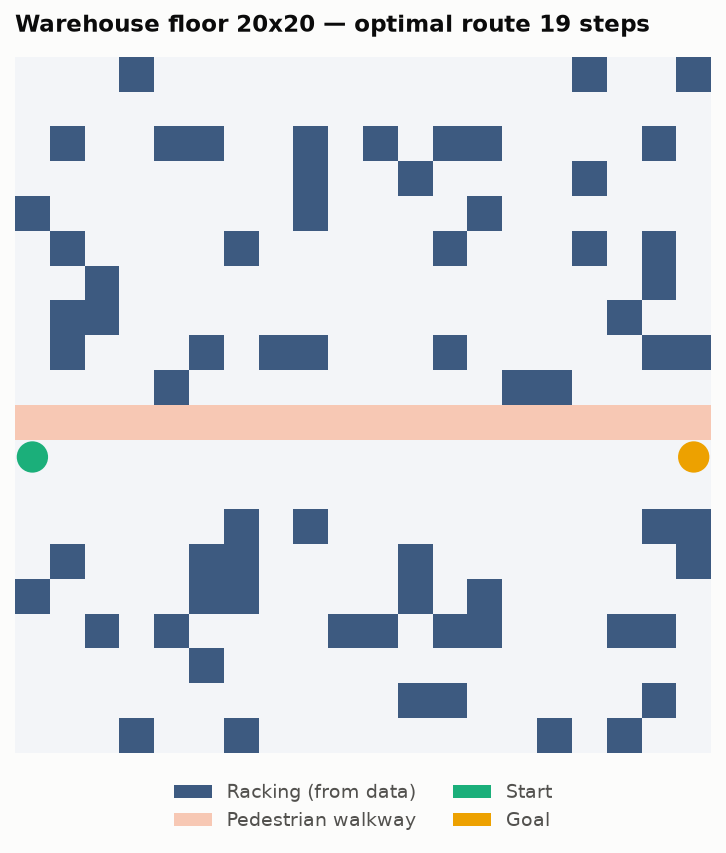
\includegraphics[width=0.66\textwidth]{figures/fig1_warehouse.png}
\caption[The warehouse floor]{The warehouse floor. Racking in dark blue comes from sixteen real
5$\times$5 dataset patches; the pale band is the pedestrian walkway. The robot travels from the
green charging station to the amber delivery point.}
\label{fig:floor}
\end{figure}

\section{The Markov decision process}
\label{sec:rewards}

\textbf{States.} The robot's cell, indexed $s = \text{row} \times W + \text{col}$, giving
$|\mathcal{S}| = 400$. The cell is a sufficient statistic for the future, so the Markov property
holds exactly.

\textbf{Actions.} The four moves recovered from the data.

\textbf{Transitions.} Deterministic. A slip probability is implemented and defaults to zero, since
the effect under study is driven by $\varepsilon$-greedy exploration rather than by environmental
stochasticity.

\textbf{Rewards.} These are the modelling assumptions:

\begin{table}[ht]
\centering
\caption[The reward structure]{The reward structure. Every value here is a declared assumption;
Chapter~\ref{ch:results} varies the one that drives the result.}
\label{tab:rewards}
\begin{tabular}{llr l}
\toprule
\textbf{Event} & \textbf{Reward} & \textbf{Effect} & \textbf{Justification} \\
\midrule
Ordinary step        & $-1$   & moves          & time costs money \\
Nudging the racking  & $-5$   & stays put      & a bump, not an incident \\
Entering the walkway & $-100$ & returned to start & a safety incident \\
Reaching the goal    & $+100$ & episode ends   & delivery completed \\
\bottomrule
\end{tabular}
\end{table}

\keypoint{Separating ``bump'' from ``incident'' is essential and was learned the hard way.} An
earlier design ended the episode on any collision. Because 17\% of the floor is racking, a random
walk struck a shelf within a few steps, every episode terminated almost immediately, and neither
algorithm ever reached the goal to discover the reward --- measured training success was 0.01.
Distinguishing a harmless bump from a genuine hazard is what makes the problem learnable while
preserving the risk structure the study requires.
